\documentclass[a4paper,conference]{IEEEtran}

% Packages
\usepackage[pdftex]{graphicx}				% Graphics
\DeclareGraphicsExtensions{.pdf,.jpeg,.jpg,.png}
\usepackage{tabularx}						% Tables
\usepackage{amsmath}						% Math
\usepackage{mathtools}						% Extra Mathematische Symbole
\usepackage{algorithmic}					% Algorithmics
\usepackage{hyperref}						% More references
\usepackage{cleveref}						% Citations
\usepackage{bytefield}						% Bytefield
\usepackage{moeptikz}						% tikz-packages for networking symbols
\usepackage{tikz}							% tikz-figures
\usetikzlibrary{decorations.pathreplacing,positioning,arrows,automata}
\tikzstyle{line} = [draw,thick,-latex]
\tikzstyle{transition} = [font=\small]

% data for figure
\begin{filecontents}{tcp.data}
#Transmission round		Congestion Window Size
1		1
2		2
3		4
4		8
5		16
6		32
7		16
8		17
9		18
10		19
11		20
12		10
13		5
14		6
15		7
\end{filecontents}


% correct bad hyphenation here
\hyphenation{op-tical net-works semi-conduc-tor}

\bibliographystyle{IEEEtran}

\begin{document}

% paper title
\title{The Origins of Congestion and\\Network-Assisted End-to-End Congestion Control}


% author
\author{\IEEEauthorblockN{Til Mohr}
\IEEEauthorblockA{RWTH Aachen University\\til.mohr@rwth-aachen.de}}

% use for special paper notices
%\IEEEspecialpapernotice{(Invited Paper)}

% make the title area
\maketitle
\IEEEpeerreviewmaketitle

\begin{abstract}
This article gives an introduction to the most common origins of network congestion. Congestion lies in different types of delay, buffer sizes, and their queue-management. While there are multiple approaches to minimize congestion, this paper will present and compare different types of algorithms used in transport protocols. TCP will be used to describe congestion avoidance, by first explaining how the protocol perceives congestion and later on how it adjusts to the current state of congestion. To compare to this approach, this paper will also take a closer look at network-assisted congestion control and a real-use implementation in data centers.
\end{abstract}

\section{Introduction}
Congestion was, is, and always will be a problem on the Internet, appearing in various forms with different symptoms causing minor but also major challenges. Most data sent over the internet is split up in smaller packets that all try to reach their destination the fastest, whether it is by taking the shortest or the least congested route. In an optimal network all computers, servers, etc. would have a direct link to each other, thus reducing the importance of bandwidth and  consequently removing the need for buffers at all. However, the larger the network grows, the number of links would increase quadratically.
\\Networks today consist of network nodes (routers, switches, ...) which all try to route internet packets as quickly as possible whilst keeping the required hardware to a minimum. Ideally, there would be a steady flow of packets being transmitted at the maximum rate. However, when an internet node receives a packet while the outgoing connection still is in use, the packet has to be stored in a buffer until the outgoing connection freed up again. Therefore, those storage units are essential to every node on a network but without proper management, even well-sized buffers could lead to network problems like packet loss, jitter, and connection delay \cite{appenzeller2004sizing}.
\\This paper will present the origins of network congestion [\autoref{sec:oc}] and analyze how TCP's congestion avoidance [\autoref{sec:ca}] protocols and network-assisted congestion control [\autoref{sec:cc}] try to avoid and minimize congestion.

\section{Origins of Congestion}
\label{sec:oc}
With the ever-growing amount of internet services not only data centers but the whole internet in general faces new challenges with each packet sent. Buffers are crucial storages inside network nodes. Their purpose is to store incoming packets while the outgoing connection is still in use. If a buffer however starts to fill up, other buffers in the same network will experience the same, thus creating congestion.
\\Therefore, a network-wide reduction of those complications is an important task to improve the quality of all internet services. While delay can cause congestion by filling up buffers, buffers itself are also an origin of congestion.

\subsection{Delay}
\label{sec:delay}
Network delay can generally speaking be categorized into four different types of delay \cite{gettys2012bufferbloat}:

\begin{figure}
	\begin{center}
	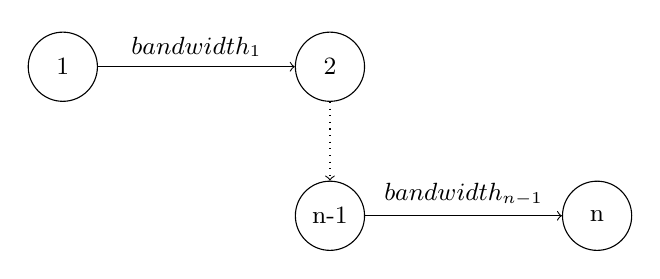
\begin{tikzpicture}[->, node distance = 1cm and 2.5cm]
		% Nodes
		\node[state] (A)  			  [transition]	{1};
		\node[state] (B) [right=of A] [transition]	{2};
		\node[state] (C) [below=of B] [transition] 	{n-1};
		\node[state] (D) [right=of C] [transition] 	{n};
		%Arrows
		\path	
		(A) edge [above] node [transition] {$bandwidth_{1}$} (B)
		(B) edge [dotted] (C)
		(C) edge [above] node [transition] {$bandwidth_{n-1}$} (D)
		;
	\end{tikzpicture}
	\end{center}
	\caption{Path a packet takes through the network. Each circle represents a network node with $1$ being the sender and $n$ being the receiver.}
	\label{fig:transmission delay}
\end{figure}

\begin{itemize}
\item 
\textit{Transmission delay} is the time it takes to send a packet from one node to another. More specifically, it describes the delay of transmitting data packets between two internet nodes depending on bandwidth and length of the connection. Typically, packets sent from an origin to a destination node are sent over various internet nodes, all of which could have a different bandwidth. Therefore, a packet send from \textbf{node 1} to \textbf{node n} over \textbf{nodes 2 to n-1} cannot be received at a faster rate than the lowest bandwidth on the path of the packet (bottleneck) [\autoref{fig:transmission delay}].\[Rate_{max} \leftarrow \min\{bandwidth_{i}\mid i\in\{1,...,n-1\}\}\]

\item
The delay known as \textit{Inter-Packet delay} describes the gap each node intentionally creates between two packets being sent. This pause is often necessary to allow the receiver to prepare for the arrival of a new packet, however, depending on the transmission protocol, other purposes may also apply.

\item
\textit{Processing delay} is the time needed to process an individual packet by an internet node. This usually means processing the packets IP header, finding its destination, and possibly queuing it in buffers.

\item
\textit{Queuing delay} is the time a packet spends waiting to be processed or transmitted.
\end{itemize}


It is important to understand that delay has a direct impact on congestion. When delay increases, the throughput of the network can decrease as packets will stay inside the network for a longer time. However, if the network continues to receive new packets at a constant rate, more and more packets will have to be stored, resulting in congestion. Generally speaking, to tackle congestion, firstly delay can be reduced, and secondly, the storages inside the network, the buffers, can be improved regarding efficient queue management and buffer size. Finally, transmission protocols can also react to congestion and adapt their send and data rate to recover from congestion [\autoref{sec:ca}] and even control congestion [\autoref{sec:cc}].
\\Whereas processing delay is almost not noticeable and transmission and inter-packet delay could be improved by upgrading cables, hardware, or transmission protocols, queuing delay has various causes and therefore is the  most difficult one to reduce. There are many different ways to implement buffers in a network node and the effectiveness of each implementation varies from where it is used. Traffic in residential network nodes, for example, differs from nodes used in large data centers in every aspect, thus hardware and software in those components should be adjusted accordingly.

\subsection{Buffers}
\label{sec:buffers}

Sizing buffers is a complex task. On the one hand, read and write times should be as short as possible to minimize additional delay. On the other hand, buffers should not be too small, as networks need to be robust for future changes and bursts and therefore nodes should store lots of data if needed while also keeping in mind the requirements of congestion detection algorithms as described in \autoref{sec:ca} to adjust for congestion appropriately \cite{staff2012bufferbloat}. Unifying those goals is very challenging as it leads to increasing costs and physical space occupied by those buffers. Additionally, a 2004 paper by Appenzeller et al. \cite{appenzeller2004sizing} found that 99\% of buffers in network nodes, which were sized on a rule-of-thumb rule based on the TCP protocol \cite{villamizar1994high}, could be removed without losing but rather gaining performance. Balancing speed and size is difficult and thus buffer sizes should be adjusted to their area of use accordingly.
\\This isn't the only major cause of queuing delay. Without proper buffer management, even nodes with well-sized buffers will experience performance loss. Proper queue management is able to compensate for the unpredictable fluidity of network traffic. It is a difficult task to buffer the right amount of packets to keep transmission flow consistent over time.
As the number of packets being transmitted grows, the \textit{throughput} of the network node increases until packets are being transmitted at the bottleneck rate. After this, the transmission rate cannot increase anymore, which leads to packets being buffered along their path to prevent them from being lost \cite{gettys2012bufferbloat}. If the incoming amount of traffic keeps exceeding the amount of outgoing traffic, those buffers will fill up (\textit{over-buffering}), which will eventually lead to \textit{bufferbloat} \cite{Allman13commentson,6886125}.

\subsubsection*{Bufferbloat}
Bufferbloat refers to frequently full and excessively large buffers in internet nodes. This leads to partly unnecessary network delay and damages congestion avoidance algorithms, such as those found in classic TCP, which will be explained in  \autoref{sec:ca} \cite{gettys2012bufferbloat,chen2014bufferbloat}. Buffering is needed to provide space to queued packets waiting for transmission resulting in a minimization of packet loss. In the past, however, buffer sizes were smaller than today's thus less packets could be queued and more were dropped, signaling transmission protocols the presence of congestion in this node early in. With memory getting cheaper over the years, buffers saw an increase in size. This has the negative impact, that more packets can be queued before any are dropped, thus those adjustments of congestion avoidance protocols kick in later than usual. Therefore, buffers are being filled in the whole network which results in an extreme increase in network delay (\textit{latency}) and fluctuation (\textit{jitter}) \cite{gettys2012bufferbloat,staff2012bufferbloat,chen2014bufferbloat}.
\\So Services, which require low latency at a high data-rate, such as streaming, will experience a decrease in quality.


\section{Congestion Avoidance}
\label{sec:ca}
\begin{figure}
\centering
\begin{bytefield}[bitheight=2.2\baselineskip ,bitwidth=0.635\baselineskip]{32}
	\bitbox{16}{Source Port} & \bitbox{16}{Destination Port} \\
	\bitbox{32}{Sequence Number} \\
	\bitbox{32}{Acknowledgment Number} \\
	\bitbox{4}{Data Offset} & \bitbox{4}{Rsrvd} &
\bitbox{1}{\tiny C\\W\\R} & \bitbox{1}{\tiny E\\C\\E} &
\bitbox{1}{\tiny U\\R\\G} & \bitbox{1}{\tiny A\\C\\K} &
\bitbox{1}{\tiny P\\S\\H} & \bitbox{1}{\tiny R\\S\\T} &
\bitbox{1}{\tiny S\\Y\\N} & \bitbox{1}{\tiny F\\I\\N} &
\bitbox{16}{Window Size} \\
\bitbox{16}{Checksum} & \bitbox{16}{Urgent Pointer} \\
\bitbox{32}{Options} \\
\bitbox{32}{Data}
\end{bytefield}
\caption{Basic structure of the TCP header. It is split up into multiple 32-bit blocks. The data block contains all the application data to be transmitted \cite{jacobson1992tcp,ietf-tcpm-rfc793bis-16,huston2000tcp}.}
\label{fig:TCP_Header}
\end{figure}
As already mentioned, congestion detection algorithms make up an important part of congestion avoidance protocols. \textit{TCP} is such a protocol, based on the transport layer, which adapts its send rate according to available network bandwidth \cite{1209197,jacobson1992tcp}. To fully understand, how TCP's congestion avoidance algorithm operates, one needs to understand how TCP works. In the following, TCP's congestion avoidance algorithm will be explained using the TCP Specification \cite{ietf-tcpm-rfc793bis-16,postel1981transmission}, also being referred to as \textit{classic TCP}. Note, there are also other TCP implementations improving upon it. The underlying concept however is the same.
\\TCP lives on the transport layer. It communicates with the application layer via sockets, splits up data into packets (and vice versa), and transmits those packets over the network with the help of the internet protocol, thus TCP is often also referred to as \textit{TCP/IP}. It is the interface between network components and computer programs. Each of those packets have different purposes but underlay the same structure - the protocol header. The TCP header is split up into multiple segments [\autoref{fig:TCP_Header}]:

\begin{itemize}
\item \textit{Source Port} and \textit{Destination Port} specify the ports on which TCP should communicate with the application layer.

\item The \textit{Sequence Numbers} and \textit{Acknowledgment Numbers} specify how much data has been sent so far. All bytes in a TCP connection are numbered in increasing order, with both sides of the connection keeping track of those numbers. This way packet loss can be detected. As the sequence numbers are limited to 32 bit, they cannot increase endlessly. Thus, if all possible sequence numbers are used up, it wraps around to 0 to keep the connection up and running \cite{postel1981transmission}.

\item TCP can set eight different bit-flags in its header. The most important one is the \textit{ACK} flag (Acknowledgement bit). Whenever a data packet arrives at its destination, a packet acknowledging the arrival of this packet will be sent back. This acknowledgment packet always has the \textit{ACK} flag set. The \textit{SYN} and \textit{FIN} flags initialize and terminate a connection.

\item The \textit{Window Size} is the maximum amount of data (in bytes) a receiver is willing to receive at any time. It is important to set it appropriately to prevent unnecessary packet loss or delay, as the receiver couldn't process the data in time. Thus, it is will also be constantly adjusted to improve the reliability of the connection \cite{jacobson1992tcp}.
\end{itemize}
TCP uses a handshake system. Whenever a client sends a data packet to the server, the server waits until it has received enough data (specified by the window size), and then sends back an acknowledgment packet, signaling the successful transmission of data. There are also other handshake operations used, for example, for establishing or terminating a connection, however, those have no further importance to the congestion avoidance protocol \cite{1209197,jacobson1992tcp,huston2000tcp,jacobson1995congestion}.

\subsection{Perceiving Congestion}
\label{sec:P_C_marker}
Both partners of a connection are both sender and receiver, as both transmit packets. In the following, however, one partner will be specified as the sender, the other as the receiver. The sender keeps track of the time it takes from when a packet sent until the acknowledgment is received. This is also known as \textit{round-trip time} (RTT). Comparing the current RTT to previously measured RTTs can inform the sender about the current state of congestion. Some variances of TCP make use of this feature in their congestion avoidance algorithms, yet classic TCP does not \cite{huston2000tcp,jacobson1995congestion}. RTT also plays a very important role in the detection of packet loss, which further implies congestion. The sender side keeps track of the RTT while it is being measured and compares it to the \textit{retransmission timeout} (RTO) \cite{jacobson1992tcp}. RTO time is being calculated by estimating the mean and variance of the RTT. Whenever packets are not acknowledged within this RTO interval, the TCP sender regards this packet as lost and will retransmit its data. Therefore, it is essential to TCP performance, that the RTO is being determined accurately, as a too low RTO could prompt unnecessary retransmissions and too high RTO could slow down the application TCP is serving \cite{huston2000tcp,jacobson1995congestion}. To implicitly notify TCP that congestion occurs, congested network nodes will occasionally drop packets after a certain threshold of queued packets has been exceeded. Usually, this is quite smaller than the maximum queue length, therefore avoiding actions can be taken in time \cite{ramakrishnan1999proposal}.

\begin{figure}
  \centering
    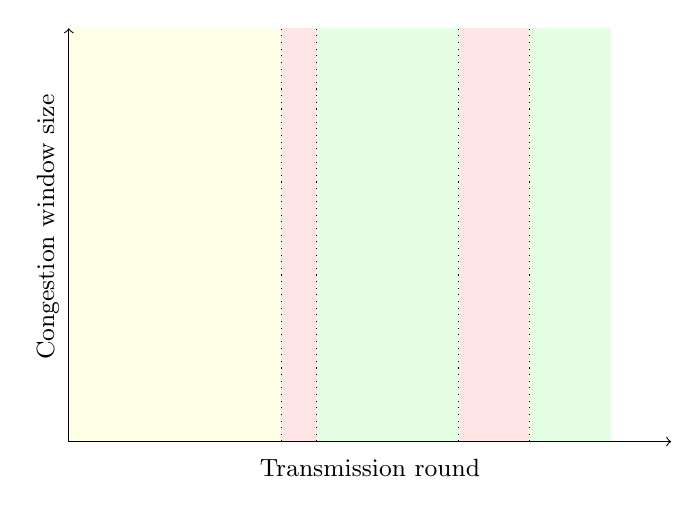
\begin{tikzpicture}[y=.15cm, x=.45cm]
    	% Ranges and dotted lines
    	\fill[yellow!10]	(0,0) rectangle (6,35);
    	\fill[red!10] 		(6,0) rectangle (7,35);
    	\fill[green!10] 	(7,0) rectangle (11,35);
    	\fill[red!10]		(11,0) rectangle (13,35);
    	\fill[green!10]		(13,0) rectangle (15.3,35);
    	\draw[dotted] 		(6,0) -- (6,35);
    	\draw[dotted] 		(7,0) -- (7,35);
    	\draw[dotted] 		(11,0) -- (11,35);
    	\draw[dotted] 		(13,0) -- (13,35);
    	% Axis
    	\draw[->] 			(0,0) -- coordinate (x axis mid) (17,0);
    	\draw[->] 			(0,0) -- coordinate (y axis mid) (0,35);
    	% Labels
    	\node[below=0.1cm] at (x axis mid) [transition] {Transmission round};
    	\node[rotate=90, above=0.1cm] at (y axis mid) [transition] {Congestion window size};
    	% Plot
    	\draw plot[mark=*]
    		file {tcp.data};
    \end{tikzpicture}
  \caption{TCP congestion avoidance protocols. Yellow represents the slow-start sequence, red and green symbolize detected congestion. The data provided is symbolic.}
  \label{fig:tcp_congestion_avoidance_protocols}
\end{figure}

\begin{figure*}[tb]
	\centering
		\begin{tikzpicture}[->, node distance = 2.5cm]
			%network
			\node[client] (H1) {};
			\node[router] (R1) [right=of H1] {};
			\node[router] (R2) [right=of R1] {};
			\node[router] (R3) [right=of R2] {};
			\node[client] (H2) [right=of R3] {};
			\path [line] (H1) -- (R1);
			\path [line] (R1) -- (R2);
			\path [line] (R2) -- (R3);
			\path [line] (R3) -- (H2);
			\path [line, dotted] (H2) -- ++(0,-35pt) -| (H1);
			\node[below=0.8cm of R2] (text) [transition] {Congested Signal};
			
			%packets
			\node[messageclosed,scale=0.8, fill=black!10] (P1) [above right=0.2cm and 1cm of H1] {};
			\node[messageclosed,scale=0.8, fill=black!50] (P2) [above left=0.7cm and 0.3cm of R2] {};
			\node[messageclosed,scale=0.8, fill=black!10] (P3) [above left=0.4cm and 0.2cm of R2] {};
			\node[messageclosed,scale=0.8, fill=black!10] (P4) [above left=0.1cm and 0.1cm of R2] {};
			\node[messageclosed,scale=0.8, fill=black!50] (P5) [above right=0.2cm and 1cm of R3] {};
			\node[above=1.5cm of R1] (P) [transition] {Packet};
			\node[above right = 1.5cm and 0.7cm of R2] (CN) [transition] {Congested Node};
			\node[above=1.5 of H2] (MP) [transition] {Marked Packet};
			\path [line] (P) -- (P1);
			\path [line] (CN) -- (R2);
			\path [line] (MP) -- (P5);
		\end{tikzpicture}
	\caption{Congestion Control Algorithm. A congested node marks buffered packets to describe congestion. This signal will be sent back to the original sender.}
	\label{fig:ecn}
\end{figure*}

\subsection{Adjusting for Congestion}
\label{sec:AfC}
To prevent congestion altogether, packet flow inside a network would have to be conservative. A connection in this state is also being described as being \textit{in equilibrium} \cite{jacobson1992tcp}. Simply speaking this means, the network works at full load whilst no additional delay or congestion is being created. However, it is quite challenging to keep a full network in this state forever. The goal of TCP's congestion avoidance algorithms, which are based on an \textit{Additive-Increase Multiplicative-Decrease} (AIMD) principle, is to react to the current state of congestion and achieve equilibrium. Those algorithms can be categorized into three sub-algorithms, that all have the goal to keep the connection in equilibrium, no matter how congestion was perceived. Here, a variable called \textit{congestion window} (cwnd) has an important role. It describes the maximum amount of data sent during an average RTT. An additional mechanism of keeping a connection in equilibrium is, that each acknowledgment packet received by the sender opens the space for a new packet to be sent into the network \cite{jacobson1992tcp}.

\subsubsection*{Slow-Start}
The \textit{slow-start} algorithm is used when a connection has just been established or when multiple packet losses were detected. The cwnd variable is set to one packet per estimated RTT because no information about network congestion has been collected yet. Whenever an acknowledgment packet is being received, cwnd will increase by one packet. This doubles cwnd each RTT, resulting in an exponential growth over time, which helps to get the packet send rate to the maximum the network can handle quite quickly, contributing to almost immediately maximum network performance \cite{jacobson1992tcp}.

\subsubsection*{Adaption}
When the network is congested, buffers in network nodes will fill up exponentially \cite{jacobson1992tcp}. Therefore, the network can only stabilize if the number of packets sent decreases at least as quickly as the queues are growing. The formula \cite{jacobson1992tcp} \[cwnd_{i+1} \leftarrow d \cdot cwnd_{i}, 0<d<1\] has an exponential decrease over time, thus resulting in the network recovering.\\
If the network isn't congested, the sender should try to raise cwnd slowly to reach the network's maximum throughput again. A multiplicative, exponential increase over time, like the slow-start algorithm isn't the best choice here. Increasing the number of packets sent drastically while cwnd still is high can challenge the network's capacity, resulting in heavy congestion. Therefore, the best option to raise cwnd to its limits is an additive increase \cite{jacobson1992tcp}:\[cwnd_{i+1} \leftarrow cwnd_{i} + u\] Van Jacobson proposes in his 1992 paper about TCP congestion avoidance that $d$ will be set to $\frac{1}{2}$ and $u$ will be set to $\frac{1}{cwnd_{i}}$. Thus, cwnd can only increase by a maximum of one packet per RTT leading to a smooth approach to the network's limit \cite{jacobson1992tcp}.

\section{Network-Assisted Congestion Control}
\label{sec:cc}
The problem that comes with classic TCP is that the congestion detection algorithms are very implicit. Packet loss, for example, may have different causes other than network congestion, such as simple cable interference, however, the congestion avoidance algorithm will still interpret it as congestion, thus possibly resulting in unnecessary network delay. Therefore, exactly determining whether the network is congested or not is crucial to keep a network stable. Here, the network layer comes into play. Because most communication should be hidden along the path of the packet, all network nodes will only communicate on the network layer (where IP lives) but not above (where TCP lives) \cite{ramakrishnan1999proposal}.\\
In 2001 a new method was standardized to explicitly notify TCP on congestion. \textit{Explicit Congestion Notification} (ECN) is an extension to TCP and IP, allowing end-to-end congestion notification while also minimizing the number of packets dropped. This is done by modifying the IP header to be able to carry one more bit - the \textit{Congestion Experienced} flag (CE) \cite{ramakrishnan1999proposal}. Instead of dropping packets occasionally after the number of queued packets exceeds a threshold [\autoref{sec:P_C_marker}], all packets supporting ECN will now be marked (setting the CE bit in the IP header) [\autoref{fig:ecn}]. Thus, congestion can be described explicitly resulting in better short- and long-term network performance. Finally, if a data packet has been marked, the according acknowledgment packet will also be marked to inform the sender of congestion \cite{ramakrishnan1999proposal,ramakrishnan2001addition,10.1145/205511.205512}.\\
To sum up so far, without ECN, classic TCP would just drive the network into congestion, and then recover from it. The network generally speaking will at least experience some jitter (fluctuating network delay). With ECN however, packets in congested nodes will be marked, explicitly informing the TCP sender that the network is congested. As a result, avoiding actions can be taken immediately. Also, the need to retransmit packets would decrease drastically, as no packets are being dropped anymore to indicate congestion. Therefore, this central principle is also being called \textit{Congestion Control} \cite{ramakrishnan1999proposal,ramakrishnan2001addition}.

\subsection{XCP}
Although TCP is a very dominant protocol on the internet, also other transport protocols could benefit from end-to-end congestion notification. The paper "Congestion Control for High Bandwidth-Delay Product Networks"  generalizes the ECN proposal of 2001, creating a new protocol called \textit{eXplicit Congestion Protocol} (XCP) while also improving upon it further by introducing new packet control concepts \cite{katabi2002congestion,1498331}. A major addition to this congestion control protocol is a feedback variable in the protocols header, which represents the amount of congestion in the network and is being computed along the data packets path.

\subsubsection*{XCP Header}
Like TCP, XCP is a window-based congestion control protocol intended for the best effort. Underneath the hood however, they are very different. A major difference between both protocols is that XCP does not only inform the sender on congestion but does also provide information about the degree of congestion. XCP can achieve this by including a \textit{congestion header} to each packet. While the sender maintains a \textit{cwnd} and \textit{RTT} variable, as with TCP, those are also being communicated to network nodes via the congestion header as \textit{H\_cwnd} and \textit{H\_rtt}. Additionally, the congestion header includes one more field. This \textit{H\_feedback} field is also initialized by the sender but is the only field that can be modified by nodes along the path \cite{katabi2002congestion,1498331}.

\subsubsection*{XCP Sender}
As with TCP, the XCP sender maintains a congestion window, \textit{cwnd}, and an estimate of the round trip time, \textit{RTT}. On packet departure, the \textit{H\_cwnd} and \textit{H\_rtt} fields will be initialized with \textit{cwnd} and \textit{RTT} accordingly. The initialization value of the \textit{H\_feedback} field represents a desired send rate $r$:
\[H\_feedback \leftarrow \frac{r \cdot RTT - cwnd}{cwnd}\]
This is an improvement to TCP's adjustment algorithms as the desired rate can be reached after one RTT.\\
The other task an XCP sender has is to adjust the congestion window according to the network's feedback. When $s$ is the packet size, the congestion window variable would be adjusted by the following formula:
\[cwnd \leftarrow \max(cwnd + H\_feedback, s)\]
In addition to responding to direct feedback, the XCP sender still needs to handle packet loss, though this is very similar to what TCP does \cite{katabi2002congestion}.

\subsubsection*{XCP Receiver}
The XCP receiver functions the same way as a TCP receiver would except for copying the (modified) congestion header from the data packet to its acknowledgment \cite{katabi2002congestion}.

\subsubsection*{XCP Router}
The main task of network nodes in XCP, or XCP routers, is to inform the XCP sender of the current state of congestion. This is done by computing feedback at every node. The objective of XCP is to prevent the queues building up to a point at which packets have to be dropped \cite{katabi2002congestion}.\\
Feedback is computed by two controllers. The \textit{Efficiency Controller} (EC) tries to maximize link utilization while minimizing queue lengths and packet drop rates. When the XCP routers link is underused, positive feedback should be sent. If the link is congested however, negative feedback should be sent to keep queue lengths minimal resulting in no packet drops \cite{katabi2002congestion,1498331}. The exact computation of feedback is beyond the scope of this paper, is however explained into detail in a paper by Wydrowsky et al. \cite{1498331}.\\
To achieve efficiency and equilibrium, this feedback will be allocated to single packets as \textit{H\_feedback}. However, the EC does not decide which packets should carry the feedback. Hence, the \textit{Fairness Controller} (FC) comes into play. As TCP, FC relies on the AIMD principle [\autoref{sec:AfC}]. If the EC calculated positive feedback, it will be split up between all packets equally. If the feedback is negative however, it will be divided between packets in proportion to their current send rates, which are determined by \textit{H\_cwnd} and \textit{H\_rtt} \cite{katabi2002congestion,1498331}.\\
Decoupling the feedback computation allows XCP to quickly acquire the maximum send rate and achieve equilibrium, all while the network allocates bandwidth to all XCP senders equally \cite{katabi2002congestion}.

\subsection{Evaluation of Network-Assisted Congestion Control}
As shown, including the network layer to detect congestion can have great performance improvements. 'Understanding XCP: Equilibrium and Fairness' has shown through simulations that many network topologies could benefit from XCP as it clears queues in equilibrium, thus resulting in improved network performance under load \cite{1498331}. Another paper has shown that XCP outperforms ordinary TCP in nearly any environment in aspects of average queue lengths, efficiency, and throughput \cite{katabi2002congestion}.
\\However, all this performance comes at a cost. Since network nodes have to actively detect congestion, ECN, XCP, and other network-assisted congestion control protocols rely on active queue management in those nodes. Although there is some hardware being produced today that meet ECNs requirements, a large part of internet hardware isn't capable of doing so. As many routers do not run on software but hardware only to improve performance, they can only handle specific packets. Whenever they cannot recognize a packet, it will simply be dropped \cite{katabi2002congestion}. So, although ECN packets differ from ordinary TCP/IP packets by only one bit, not all routers can handle this change and will drop those packets. This is the reason you do not see these kinds of protocols in wide area networks (WAN) too often, let alone the internet.
\\Nevertheless, whenever the implementation of XCP, ECN, or similar protocols is not a challenge, can implement network-assisted congestion control with ease and see great performance improvements. Especially smaller networks with high traffic could benefit from those technologies [\autoref{sec:DCTCP}].

\subsection{DCTCP}
\label{sec:DCTCP}
A lot of internet services run in data centers with large amounts of computers communicating with each other, resulting in a lot of traffic inside the data center. Optimizing those data centers networking capabilities can increase application productivity. In 2010 a paper proposed \textit{DCTCP}, a variation of TCP using ECN to create a data transportation protocol, which especially takes hardware purposed for use in those environments into account \cite{10.1145/1851275.1851192}.\\
The general problem that appears in high-traffic environments is the so-called \textit{TCP Incast} problem. It describes a drastic reduction in application throughput. To understand where TCP incast originates, one fist needs to understand how most data centers are built. A typical data center contains a set of racks, each holding a large number of servers, the switches, that connect those racks, and connecting links, that connect those switches to other parts of the data center or the internet [\autoref{fig:dc}]. This design pattern is also known as \textit{Partition/Aggregate} and is most commonly used in data centers. It however results in a high 'fan-in', as multiple servers (leaves) are connected to just one link (root) \cite{10.1145/1851275.1851192,10.1145/1592681.1592693}. Additionally, most applications require high bandwidth, low latency connections, also enabling them to send many parallel requests to other servers. Combining those requirements with the design pattern, it becomes clear, that those switches are being challenged. Besides, many data center switches have relatively small, shared buffers. Therefore, it is common that many packets are being transmitted at the same time (\textit{bursty retransmissions}), resulting in a collapse of throughput \cite{10.1145/1851275.1851192,10.1145/1592681.1592693}.\\
The goal of DCTCP is to keep data center traffic constantly flowing, which means meeting the requirements applications take while keeping relatively small buffer sizes inside switches in mind. To achieve this, DCTCP implements ECN. Unlike TCP however, if a DCTCP sender registers congestion, the window size will be reduced by a fraction of the number of marked packets it received. Therefore, excessive link underutilization can be prevented. In addition, the DCTCP receiver will only send one ACK packet for every $m$ consecutive data packet, where all $1,...,m$ packets before had the same CE-flag configuration. Here, $m$ is a variable initialized while the DCTCP connection is being established and cannot be changed without renegotiation. Therefore, fewer packets are sent through the network but the TCP sender is still able to identify lost packets and register congestion \cite{10.1145/1851275.1851192}.
\\However, being a bandwidth greedy transmission protocol, data centers using DCTCP can see a performance drop when they additionally use other transmission protocols such as TCP or ECN. As DCTCP tries to utilize the links as much as possible, non-greedy protocols will be neglected and will see a drop in performance. Thus, data centers should avoid using DCTCP in addition to other protocols to fully make use of DCTCP's capabilities.
\\To sum up, being able to react to congestion immediately enables DCTCP to reduce buffer overflows and timeouts, thus largely resolving incast problems. The paper proposing DCTCP has found, that their protocol increases traffic by 110\% while using 90\% less buffer space compared to TCP \cite{10.1145/1851275.1851192}. Therefore it is unsurprising that DCTCP is very popular in data centers.

\begin{figure}
	\centering
		\begin{tikzpicture}[node distance = 2.5cm]
			\node[router, scale=0.8] (Router) {};
			\node (Internet) [right = 1.5cm of Router, text width=2cm] {Outgoing Connection};
			\node[switch, scale=0.8] (Sw1) [below left = 0.8cm and 1cm of Router] {};
			\node[switch, scale=0.8] (Sw2) [below right = 0.8cm and 1cm of Router] {};
			\node[server, scale=1] (S1) [below left = 0.8cm and 0.25cm of Sw1] [transition] {Server};
			\node[server, scale=1] (S2) [below = 2.1cm of Router] [transition] {Server};
			\node[server, scale=1] (S3) [below right = 0.8cm and 0.25cm of Sw2] [transition] {Server};
			
			\draw[-] (Router) -- (Sw1);
			\draw[-] (Router) -- (Sw2);
			\draw[-, dotted] (Router) -- (Internet);
			\draw[-] (Sw1) -- (S1);
			\draw[-] (Sw1) -- (S2);
			\draw[-] (Sw1) -- (S3);
			\draw[-] (Sw2) -- (S1);
			\draw[-] (Sw2) -- (S2);
			\draw[-] (Sw2) -- (S3);
			
			\draw[decorate,decoration={brace,amplitude=10pt},xshift=-4pt,yshift=0pt] (S1.north -| S1.west) -- (Router.center -| S1.west) node [black,midway,xshift=-1cm,align=right] [transition] {High\\ 'Fan-In'};
		\end{tikzpicture}
	\hspace{1cm}
	\caption{Data Center High 'Fan-In'}
	\label{fig:dc}
\end{figure}

\section{Conclusion}
This paper has analyzed the origins of congestion. Different factors play a role in network congestion, however, especially full buffers at congested nodes will cause traffic delay. Further, we assess the functionality of congestion avoidance algorithms, especially classic TCP. However, since those algorithms quite often do cause network stress rather than resolving it, we took a closer look at network-assisted end-to-end congestion control. ECN, an addition to TCP, and XCP are two standardized protocols applying those principles but haven't been very successful in wide area networks (WAN). In smaller networks, the implementation of them is easier. DCTCP, a variation of ECN, as an example, can successfully resolve many issues occurring in data centers.

\bibliography{references}

\end{document}
